\section{Date: 2026-11-14}
\noindent \textbf{Series ID: FDHBFRB} 

\noindent This series is titled Federal Debt Held by Federal Reserve Banks (DISCONTINUED) and has a frequency of Quarterly, End of Period. The units are Billions of Dollars and the seasonal adjustment is Seasonally Adjusted.The observation start date is 1953-01-01 and the observation end date is 1998-10-01.The popularity of this series is 3. \\ 

\noindent \textbf{Series ID: U13SMI} 

\noindent This series is titled Manufacturers' Materials and Supplies Inventories: Textile Mills and has a frequency of Monthly, End of Period. The units are Millions of Dollars and the seasonal adjustment is Not Seasonally Adjusted.The observation start date is 1992-01-01 and the observation end date is 2026-09-01.The popularity of this series is 1. \\ 

\subsection{Raw Regression}
\noindent Regresses the two series against each other directly. A significant result here can come just as easily from both series sharing a long-run trend as from any real relationship.

\begin{center}
\begin{tabular}{lclc}
\toprule
\textbf{Dep. Variable:}       & value\_fred\_U13SMI & \textbf{  R-squared:         } &     0.645   \\
\textbf{Model:}               &         OLS         & \textbf{  Adj. R-squared:    } &     0.632   \\
\textbf{Method:}              &    Least Squares    & \textbf{  F-statistic:       } &     47.29   \\
\textbf{Date:}                &   Sat, 14 Nov 2026  & \textbf{  Prob (F-statistic):} &  2.67e-07   \\
\textbf{Time:}                &       17:23:21      & \textbf{  Log-Likelihood:    } &   -166.92   \\
\textbf{No. Observations:}    &            28       & \textbf{  AIC:               } &     337.8   \\
\textbf{Df Residuals:}        &            26       & \textbf{  BIC:               } &     340.5   \\
\textbf{Df Model:}            &             1       & \textbf{                     } &             \\
\textbf{Covariance Type:}     &      nonrobust      & \textbf{                     } &             \\
\bottomrule
\end{tabular}
\begin{tabular}{lcccccc}
                              & \textbf{coef} & \textbf{std err} & \textbf{t} & \textbf{P$> |$t$|$} & \textbf{[0.025} & \textbf{0.975]}  \\
\midrule
\textbf{const}                &    1208.6362  &      129.308     &     9.347  &         0.000        &      942.840    &     1474.432     \\
\textbf{value\_fred\_FDHBFRB} &       2.3512  &        0.342     &     6.876  &         0.000        &        1.648    &        3.054     \\
\bottomrule
\end{tabular}
\begin{tabular}{lclc}
\textbf{Omnibus:}       &  1.056 & \textbf{  Durbin-Watson:     } &    1.030  \\
\textbf{Prob(Omnibus):} &  0.590 & \textbf{  Jarque-Bera (JB):  } &    0.223  \\
\textbf{Skew:}          &  0.085 & \textbf{  Prob(JB):          } &    0.895  \\
\textbf{Kurtosis:}      &  3.402 & \textbf{  Cond. No.          } & 2.66e+03  \\
\bottomrule
\end{tabular}
%\caption{OLS Regression Results}
\end{center}

Notes: \newline
 [1] Standard Errors assume that the covariance matrix of the errors is correctly specified. \newline
 [2] The condition number is large, 2.66e+03. This might indicate that there are \newline
 strong multicollinearity or other numerical problems.

\begin{figure}
\centering
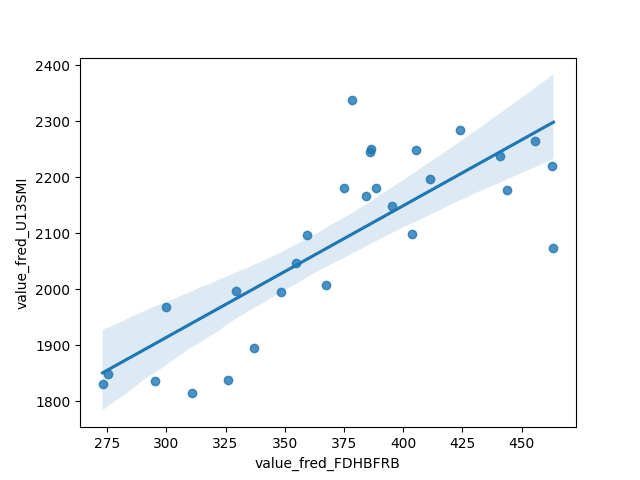
\includegraphics[scale = 0.9]{plots/plot_2026-11-14.png}
\caption{Raw Regression Plot for 2026-11-14}
\end{figure}
\newpage
\subsection{Detrended Regression}
\noindent Regresses the residuals of each series after removing its own linear time trend, so a shared trend can no longer drive the result on its own. A relationship that stays significant here is better evidence of a genuine link between the two series.

\begin{center}
\begin{tabular}{lclc}
\toprule
\textbf{Dep. Variable:}                  & value\_fred\_U13SMI\_detrended & \textbf{  R-squared:         } &     0.024   \\
\textbf{Model:}                          &              OLS               & \textbf{  Adj. R-squared:    } &    -0.014   \\
\textbf{Method:}                         &         Least Squares          & \textbf{  F-statistic:       } &    0.6308   \\
\textbf{Date:}                           &        Sat, 14 Nov 2026        & \textbf{  Prob (F-statistic):} &    0.434    \\
\textbf{Time:}                           &            17:23:21            & \textbf{  Log-Likelihood:    } &   -166.72   \\
\textbf{No. Observations:}               &                 28             & \textbf{  AIC:               } &     337.4   \\
\textbf{Df Residuals:}                   &                 26             & \textbf{  BIC:               } &     340.1   \\
\textbf{Df Model:}                       &                  1             & \textbf{                     } &             \\
\textbf{Covariance Type:}                &           nonrobust            & \textbf{                     } &             \\
\bottomrule
\end{tabular}
\begin{tabular}{lcccccc}
                                         & \textbf{coef} & \textbf{std err} & \textbf{t} & \textbf{P$> |$t$|$} & \textbf{[0.025} & \textbf{0.975]}  \\
\midrule
\textbf{const}                           &   -1.438e-10  &       18.288     & -7.87e-12  &         1.000        &      -37.591    &       37.591     \\
\textbf{value\_fred\_FDHBFRB\_detrended} &       1.3426  &        1.690     &     0.794  &         0.434        &       -2.132    &        4.817     \\
\bottomrule
\end{tabular}
\begin{tabular}{lclc}
\textbf{Omnibus:}       &  1.455 & \textbf{  Durbin-Watson:     } &    0.973  \\
\textbf{Prob(Omnibus):} &  0.483 & \textbf{  Jarque-Bera (JB):  } &    0.437  \\
\textbf{Skew:}          &  0.123 & \textbf{  Prob(JB):          } &    0.804  \\
\textbf{Kurtosis:}      &  3.561 & \textbf{  Cond. No.          } &     10.8  \\
\bottomrule
\end{tabular}
%\caption{OLS Regression Results}
\end{center}

Notes: \newline
 [1] Standard Errors assume that the covariance matrix of the errors is correctly specified.

\begin{figure}
\centering
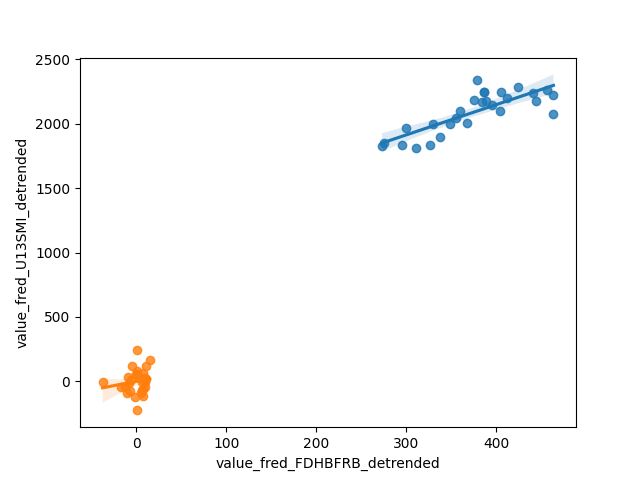
\includegraphics[scale = 0.9]{plots/plot_2026-11-14_detrended.png}
\caption{Detrended Regression Plot for 2026-11-14}
\end{figure}
\newpage
